%
% chapter.tex -- Beschreibung des Inhaltes
%
% (c) 2021 Prof Dr Andreas Müller, Hochschule Rapperswil
%
% !TeX spellcheck = de_CH
\chapter{Spezielle Funktionen und Rekursion
\label{buch:chapter:rekursion}}
\lhead{Spezielle Funktionen und Rekursion}
\rhead{}

%
% gamma.tex -- Abschnitt über die Gamma-funktion
%
% (c) 2021 Prof Dr Andreas Müller, OST Ostschweizer Fachhochschule
%
\section{Die Gamma-Funktion
\label{buch:rekursion:section:gamma}}
\rhead{Gamma-Funktion}
Die Fakultät $x!$ kann rekursiv durch 
\[
	x! = x\cdot (x-1)! \qquad\text{und}\qquad 0!=1
\]
für alle natürlichen Zahlen $x\in\mathbb{N}$ definiert werden.
Äquivalent damit ist eine Funktion 
\begin{equation}
\Gamma(x+1) = x\Gamma(x)
\qquad\text{und}\qquad 
\Gamma(1)=1.
\label{buch:rekursion:eqn:gammadef}
\end{equation}
Kann man eine reelle oder komplexe Funktion finden, die die
Funktionalgleichung~\eqref{buch:rekursion:eqn:gammadef}
erfüllt und damit die Fakultät auf beliebige Argumente ausdehnt?

\subsection{Produktformel}
Die Fakultät $n!$ ist ein Produkt von $n$ Faktoren, es ist daher
natürlich zu versuchen, auch $x!$ als ein Produkt zu schreiben.
Allerdings kann es nicht möglich sein, dies mit einer endlichen
Anzahl von Faktoren zu machen, denn wenn $x$ grösser wird, muss auch
die Zahl der Faktoren grösser werden.
Mit jedem zusätzlichen Faktor ist ein Sprung der Werte zu erwarten.
Wir erwarten daher entweder ein unendliches Produkt oder einen
Ausdreck, bei dem die ``Anzahl'' $x$ der Faktoren im Exponenten
steht.
In diesem Abschnitt soll zunächst eine solcher Ausdruck gefunden
werden.
Dieser ist jedoch für die numerische Berechnung absolut ungeeignet,
so dass er später in ein unendliches Produkt umgeformt werden muss.

\subsubsection{Fakultät als Bruch}
Euler hat das Problem, die Fakultät auf beliebige reelle oder komplexe
Zahlen auszudehnen, wie folgt angepackt.
Zunächst hat er bemerkt, dass für ganzzahlige $x$ und natürliche $n$
\begin{align}
x! 
&=
1\cdot 2\cdot 3\cdot\ldots\cdot x
\notag
\\
&=
\frac{
1\cdot 2\cdot 3\cdot\ldots\cdot x\cdot (x+1) (x+2)\cdots(x+n)
}{
(x+1)(x+2)\cdots(x+n)
}
\notag
\\
&=
\frac{
1\cdot 2\cdot\ldots\cdot n\cdot(n+1)\cdot(n+2)\cdots(n+x)
}{
(x+1)(x+2)\cdots(x+n)
}
\notag
\\
&=
\frac{n! \cdot (n+1)(n+1)\cdots(n+x)}{(x+1)(x+2)\cdots(x+n)}
\label{buch:rekursion:gamma:eqn:fakultaet}
\end{align}
gilt.
Der Plan ist, dies so umzuformen, dass man für $x$ eine beliebige
komplexe Zahl einsetzen kann.

\subsubsection{Pochhammer-Symbol}
Die spezielle Form des Nenners und des zweiten Faktors im Zähler
von \eqref{buch:rekursion:gamma:eqn:fakultaet}
rechtfertigt die folgende Definition.

\begin{definition}[Pochhammer]
Für $a\in\mathbb{C}$ und $n\in\mathbb{N}$ heisst das Produkt
\[
(a)_n = a\cdot(a+1)\cdot(a+2)\cdots(a+n-1)
\]
das Pochhammer-Symbol oder die verschobene Fakultät.
\index{Pochhammer-Symbol}
\end{definition}

Die verschobene Fakultät $(a)_n$ hat also genau $n$ Faktoren, deren
erster $1$ ist.
Die gewöhnliche Fakultät hat $n$ Faktoren, deren erster $1$ ist, also
ist $n! = (1)_n$.

Der Ausdruck \eqref{buch:rekursion:gamma:eqn:fakultaet}
für $x!$ wird unter Verwendung des Pochhammer-Symbols zu
\begin{equation}
x! = \frac{n! (n+1)_x}{(x+1)_n}.
\label{buch:rekursion:gamma:eqn:produkt2}
\end{equation}
Leider ist dieser Ausdruck ebenfalls nicht auf beliebige $x$
verallgemeinerungsfähig, denn $(n)_x$ ist nur natürliche $x$ definiert.
Der Faktor $(n+1)_x$ enthält $x$ Faktoren beginnend bei $n$.
Für grosses $n$ sind diese Faktoren nahe beeinander, man sollte also
$(n+1)_x$ durch $n^x$ approximieren können.
Wir erweitern daher \eqref{buch:rekursion:gamma:eqn:produkt2} mit $n^x$
und erhalten
\begin{equation}
x!
=
\frac{n!\,n^x}{(x+1)_n}\cdot
\frac{(n+1)_x}{n^x}.
\label{buch:rekursion:gamma:eqn:produkt3}
\end{equation}
Der erste Faktor in diesem Ausdruck enthält jetzt nur noch Dinge,
die für beliebige $x\in\mathbb{C}$ definiert sind.

\subsubsection{Grenzwertdefinition}
Der zweite Bruch in \eqref{buch:rekursion:gamma:eqn:produkt3}
besteht aus Termen, die zwar nur für natürliches $x$ definiert sind,
wir vermuten aber, dass er für grosses $n$ gegen $1$ konvergiert.
Tatsächlich gilt
\[
\lim_{n\to\infty}
\frac{(n+1)_x}{n^x}
=
\lim_{n\to\infty}
\underbrace{\frac{n+1}{n}}_{\displaystyle\to 1}
\cdot
\underbrace{\frac{n+2}{n}}_{\displaystyle\to 1}
\cdot\ldots\cdot
\underbrace{\frac{n+x}{n}}_{\displaystyle\to 1}
=
1,
\]
da  $(n+x)/n=1+x/n\to 1$ für grosses $n$.
Dies würde die folgende Definition rechtfertigen.

\begin{definition}
\label{buch:rekursion:gamma:def:definition}
Die Gamma-Funktion $\Gamma(x)$ einer Zahl
$x\in\mathbb{C}\setminus\{0,-1,-2,-3,\dots\}$ ist der Grenzwert
\[
\Gamma(x) = \lim_{n\to\infty} \frac{n!\,n^{x-1}}{(x)_n}.
\] 
\end{definition}

\subsubsection{Rekursionsgleichung für $\Gamma(x)$}
Es ist aus der Herleitung klar, dass $\Gamma(n)=(n-1)!$ sein muss.
Wir sollten dies aber auch direkt aus der
Definition~\ref{buch:rekursion:gamma:def:definition} ableiten
können.
Dazu müssen wir nur überprüfen, ob $\Gamma(1)=0!=1$ ist und ob
die Rekursionsformel $\Gamma(n)=n\Gamma(n-1)$ gilt.

Den Wert $\Gamma(1)$ kann man direkt berechnen:
\[
\Gamma(1)
=
\lim_{n\to\infty} \frac{n!}{(1)_n}
=
\lim_{n\to\infty} \frac{n!}{n!}
=
1
\]
wegen $(1)_n=n!$.

Für die Rekursionsformel muss man den Grenzwert für $x$ und $x+1$
miteinander vergleichen.
Aus dem Term $(x+1)_n$ im Nenner muss man einen Term $(x)_n$ machen,
dies ist möglich, indem man mit $x$ erweitert:
\begin{align*}
\Gamma(x+1)
&=
\lim_{n\to\infty}\frac{n!\,n^x}{(x+1)_n}
=
x\lim_{n\to\infty}\frac{n!\,n^x}{x(x+1)_n}
=
x\lim_{n\to\infty}\frac{n!\,n^x}{(x)_{n+1}}.
\intertext{Wir müssen jetzt nur noch zeigen, dass der Grenzwert
auf der rechten Seite gegen $\Gamma(x)$ konvergiert,
in dessen Definition aber die Potenz $n^{x-1}$ vorkommt.
Wir müssen also einen Faktor $n$ los werden und gleichzeitig
aus $n$ überall $n+1$ machen, damit der Nenner wieder passt.
Dabei wird}
\Gamma(x+1)
&=
x\lim_{n\to\infty}
\frac{(n+1)!n^{x-1}}{(x)_{n+1}}
\cdot
\underbrace{\frac{n}{n+1}}_{\displaystyle\to 1}
\\
&=
x\lim_{n\to\infty}
\underbrace{\frac{(n+1)!(n+1)^{x-1}}{(x)_{n+1}}}_{\displaystyle\to\Gamma(x)}
\cdot
\frac{n^{x-1}}{(n+1)^{x-1}}
\\
&=
\Gamma(x)
\lim_{n\to\infty} \biggl(\frac{n}{n+1}\biggr)^{x-1}
=
\Gamma(x),
\end{align*}
Weil $n/(n+1)\to 1$ ist und die Funktion $z\mapsto z^{x-1}$ für alle
nach der Definition zulässigen Werte von $x$ eine stetige Funktion ist.

\subsubsection{Numerische Unzulänglichkeiten der Grenzwertdefinition}
Die Grenzwertdefinition~\ref{buch:rekursion:gamma:def:definition}
ist zwar zweifellos richtig, kann aber nicht für die numerische 
Berechnung der Gamma-Funktion verwendet werden.
Die Existenz des Grenzwertes verwendet, dass $x\ll n$ sein muss,
damit $(n+x)/n$ gegenüber $1$ vernachlässigt werden kann.
Die Grenzwertdefinition beginnt also erst, vernünftige Approximationen
von $\Gamma(x)$ zu geben, wenn $n$ viel grösser also $x$ ist.
Andererseits wächst $n!$ sehr schnell an, schon für $n=171$ ist
das Resultat grösser als was der \texttt{double}-Datentyp fassen kann.
Dies ist aber viel zu kleine, um gute Approximationen auch für kleine
Werte von $x$ zu geben.
So findet man zum Beispiel für $x=\frac12$ und $n=170$ mit Octave
\[
\frac{n!\,n^{x-1}}{(x)_n}
=
\frac{170!}{\sqrt{170}\cdot \frac12\cdot\frac32\cdot\ldots\cdot\frac{339}{2}}
=
\frac{7.2574\cdot10^{307}}{13.308\cdot 3.1381\cdot10^{305}}
=
1.7738.
\]
Andererseits werden wir später sehen, dass 
\[
\Gamma({\textstyle\frac12})
=
\sqrt{\pi}
=
1.772453850905516
\]
ist.
Die Approximation mit Hilfe der Grenzwertdefinition kann also
grundsätzlich nicht mehr als zwei korrekte Nachkommastellen liefern.

\subsubsection{Produktformel}
Ein möglicher Ausweg aus den numerischen Schwierigkeiten mit der
Grenzwertdefinition ist, den schnell wachsenden Faktor $n!$
in den Zähler zu bringen, so dass er der Konvergenz etwas nachhilft.
Wir berechnen daher den Kehrwert $1/\Gamma(x)$.

\begin{satz}
\label{buch:rekursion:gamma:satz:produktformel}
Der Kehrwert der Gamma-Funktion kann geschrieben werden als
\begin{equation}
\frac{1}{\Gamma(x)}
=
xe^{\gamma x}
\prod_{k=1}^\infty
\biggl(1+\frac{x}k\biggr)\,e^{-\frac{x}{k}},
\label{buch:rekursion:gamma:eqn:produktformel}
\end{equation}
wobei $\gamma$ die Euler-Mascheronische Konstante
\[
\gamma
=
\lim_{n\to\infty}
\biggl(\sum_{k=1}^n\frac{1}{k}-\log n\biggr)
\]
ist.
\end{satz}

\begin{proof}[Beweis]
Es sind zwei Dinge nachzuprüfen.
Zunächst muss nachgewiesen werden, dass das unendliche Produkt 
überhaupt konvergiert.
Wenn das gesichert ist, muss noch gezeigt werden, dass der Grenzwert
tatsächlich $1/\Gamma(x)$ ist.

Für die Konvergenz beachtet man, dass die Faktoren des Produkts 
die Form
\begin{align*}
\biggl(1+\frac{x}n\biggr)e^{-\frac{x}{n}}
&=
\biggl(1+\frac{x}n\biggr)
\biggl(1-\frac{x}{n}+\frac{x^2}{2n^2}-\frac{x^3}{3!n^3}+\dots\biggr)
\\
&=
1-\frac{x^2}{n^2} + 
\biggl(1+\frac{x}n\biggr)
\biggl(\frac{x^2}{2n^2}-\dots\biggr)
\\
&=
1-\frac{x^2}{n^2} + \frac{x^2}{2n^2} + O\bigl((\textstyle\frac{x}{n})^2\bigr)
\\
&=
1-\frac{x^2}{2n^2} + O\bigl((\textstyle\frac{x}{n})^3\bigr)
\end{align*}
haben.
Da die Reihe 
\[
\sum_{n=1}^\infty \frac{x^2}{n^2}
\]
konvergent ist, konvergiert auch das Produkt.
% XXX wir brauchen irgendwo das Konvergenzkriterium für ein Produkt

Um die Übereinstimmung der Produktformel mit $1/\Gamma(x)$ zu zeigen,
berechnen wir
\begin{align*}
\frac{1}{\Gamma(x)}
&=
\lim_{n\to\infty} 
\frac{(x)_n}{n!\,n^{x-1}}
=
\lim_{n\to\infty} 
\frac{x(x+1)(x+2)\cdots(x+n-1)}{1\cdot 2\cdot3\cdots (n-1)\cdot n\cdot n^{x-1}}
\\
&=
x
\lim_{n\to\infty} 
\frac{x+1}{1}
\cdot
\frac{x+2}{2}
\cdots
\frac{x+n-1}{n-1}
\cdot
n^{-x}
\\
&=
x
\lim_{n\to\infty}
\biggl(1+\frac{x}{1}\biggr)
\cdot
\biggl(1+\frac{x}{2}\biggr)
\cdots
\biggl(1+\frac{x}{n-1}\biggr)
\cdot
e^{-x\log n}
\\
&=
x
\prod_{k=1}^{n-1}
\biggl(1+\frac{x}{k}\biggr)
e^{-\frac{x}{k}}
e^{\frac{x}{k}}
e^{-x\log n}
\\
&=
x
\biggl(
\lim_{n\to\infty}
\prod_{k=1}^{n-1}
\biggl(1+\frac{x}{k}\biggr)
e^{-\frac{x}{k}}
\biggr)
\cdot
\biggl(
\lim_{n\to\infty}
e^{x\bigl(\sum_{k=1}^{n-1}\frac{1}{k} - \log n\bigr)}
\biggr)
\end{align*}
Der Klammerausdruck im Exponent des letzten Faktors auf der rechten Seite
konvergiert nach Definition der Euler-Mascheronischen Konstanten gegen
$\gamma$, somit folgt 
\[
\frac{1}{\Gamma(x)}
=
xe^{\gamma x}\prod_{k=1}^\infty \biggl(1+\frac{x}{k}\biggr)e^{-\frac{x}{k}},
\]
wie behauptet.
Damit ist Satz~\ref{buch:rekursion:gamma:satz:produktformel}
vollständig bewiesen.
\end{proof}

\begin{table}
\centering
\begin{tabular}{|>{$}c<{$}|>{$}c<{$}|>{$}c<{$}|}
\hline
k &  \Gamma(\frac12,n) & \Gamma(\frac12) - \Gamma(\frac12,n) \\
\hline
1 & 1.\underline{7}518166478 & -0.0206372031 \\
2 & 1.\underline{77}02543372 & -0.0021995137 \\
3 & 1.\underline{772}2324556 & -0.0002213953 \\
4 & 1.\underline{7724}316968 & -0.0000221541 \\
5 & 1.\underline{77245}16354 & -0.0000022156 \\
6 & 1.\underline{772453}6293 & -0.0000002216 \\
\hline
\end{tabular}
\caption{Werte $\Gamma(\frac12,n)$ von $\Gamma(\frac12)$ berechnet mit
$n=10^k$ Faktoren der
Produktformel~\eqref{buch:rekursion:gamma:eqn:produktformel}
und der zugehörige Fehler.
Die korrekten Nachkommastellen sind unterstrichen.
\label{buch:rekursion:gamma:gammatabelle}}
\end{table}

Um zu zeigen, dass die Produktform tatsächlich besser geeignet ist,
sind in der Tabelle~\ref{buch:rekursion:gamma:gammatabelle}
die Resultate der numerischen Rechnung  bis $n=1000000$ zusammengestellt.
Die Produktformel kann gute Werte von $\Gamma(x)$ auch für derart grosse
Werte von $n$ problemlos berechnen.

Der Fehler der numersichen Approximation ist von der Grössenordnung
$O(1/n)$ wie das auf Grund des verwendeten Konvergenzkriteriums
zu erwarten war.
Die Anzahl zu berücksichtigender Terme wächst daher exponentiall
mit der Anzahl gewünschter Stellen an, was für praktische Zwecke
zu langsam ist.
Für die numersiche Berechnung der Gamma-Funktion ist die Produktformel
daher im Allgemeinen nicht geeignet.

%
% Integralformel für die Gamma-Funktion
%
\subsection{Integralformel für die Gamma-Funktion}
Euler hat die folgende Integraldefinition der Gamma-Funktion gegeben.

\begin{definition}
\label{buch:rekursion:def:gamma}
Die Gamma-Funktion ist die Funktion 
\[
\Gamma
\colon
\{z\in\mathbb{C} \mid \operatorname{Re}z>0\}
\to \mathbb{C}
:
z
\mapsto
\Gamma(z) = \int_0^\infty t^{z-1}e^{-t}\,dt
\]
\end{definition}

Man beachte, dass das Integral für $x=0$ nicht definiert ist, eine
Potenzreihenentwicklung um einen Punkt $x_0$ auf der positiven reellen
Achse kann also höchstens den Konvergenzradius $\varrho=|x_0|$ haben.

\begin{figure}
\centering
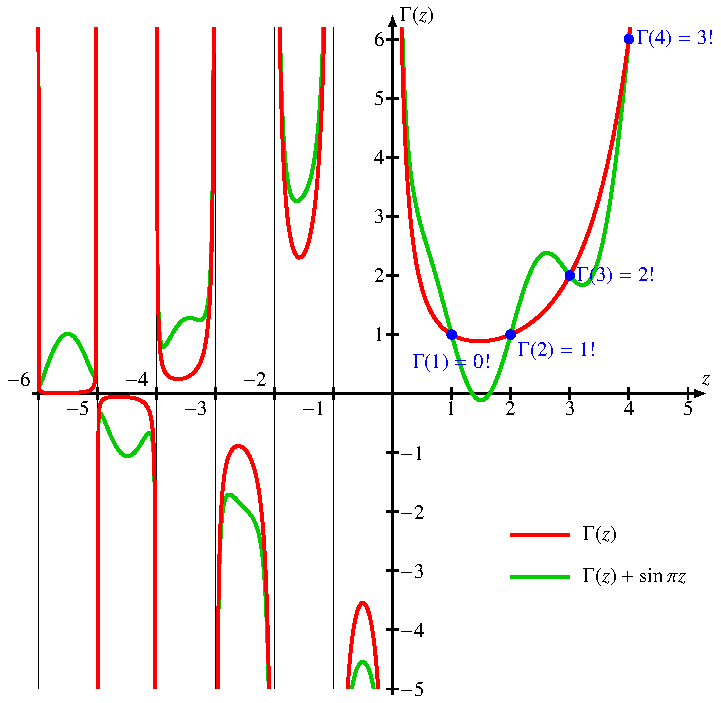
\includegraphics{chapters/040-rekursion/images/gammaplot.pdf}
\caption{Graph der Gamma-Funktion $z\mapsto\Gamma(z)$ und der alternativen
Funktion $\Gamma(z)+\sin(\pi z)$, die für ganzzahlige Argumente ebenfalls
die Werte der Fakultät annimmt.
\label{buch:rekursion:fig:gamma}}
\end{figure}

\subsubsection{Alternative Lösungen}
Die Funktion $\Gamma(z)$ ist nicht die einzige Funktion, die natürlichen
Zahlen die Werte $\Gamma(n+1) = n!$ der Fakultät annimmt.
Indem man eine beliebige Funktion $f(z)$ addiert, die auf alle
natürlichen Zahlen verschwindet, also $f(n)=0$ für $n\in\mathbb{N}$,
erhält man eine weitere Funktion, die auf natürlichen Zahlen
die Werte der Fakultät annimmt.
Ein Beispiel einer solchen Funktion ist
\begin{equation}
z\mapsto f(z)=\Gamma(z) + \sin \pi z,
\label{buch:rekursion:eqn:gammaalternative}
\end{equation}
die Funktion $f(z)=\sin\pi z$ verschwindet sogar auf allen ganzen
Zahlen.

In Abbildung~\ref{buch:rekursion:fig:gamma} ist die Gamma-Funktion
in rot geplotet, die Funktion~\eqref{buch:rekursion:eqn:gammaalternative}
in grün.
Die Punkte $(n,(n-1)!)$ sind in blau bezeichnet, sie sind beiden Graphen
gemeinsam.

\subsubsection{Pol erster Ordnung bei $z=0$}
Wir haben zu prüfen, dass sowohl der Wert $\Gamma(1)$ korrekt ist als
auch die Rekursionsformel~\eqref{buch:rekursion:eqn:gammadef} gilt.
Der Wert für $z=1$ ist
\begin{align*}
\Gamma(1)
&=
\int_0^\infty t^{1-1}e^{-t}\,dt
=
\left[ -e^{-t} \right]_0^\infty
=
1.
\end{align*}
Für die Rekursionsformel kann mit Hilfe von partieller Integration
bekommen:
\begin{align*}
\Gamma(z+1)
&=
\int_0^\infty t^{z+1-1}e^{-t}\,dt
=
\biggl[-t^{z}e^{-t}\biggr]_0^\infty
+
\int_0^\infty z t^{z-1}e^{-t}\,dt
\\
&=
z
\int_0^\infty
t^{z-1}e^{-t}\,dt
=
z \Gamma(z).
\end{align*}

Für $0<z<\varepsilon$ für eine $\varepsilon >0$ folgt aus der 
Funktionalgleichung
\[
\Gamma(z) = \frac{\Gamma(1+z)}{z}.
\]
Da $\Gamma(1)=1$ ist und $\Gamma$ eine in einer
Umgebung von $1$ stetige Funktion ist, kann sie in der Form
\(
\Gamma(1+z)=\Gamma(1) + zf(z)
\)
schreiben, wobei  $f(z)$ eine differenzierbare Funktion ist mit
$f'(1)=\Gamma'(1)$.
Daraus ergibt sich für $\Gamma(z)$ der Ausdruck
\[
\Gamma(z) = \frac{\Gamma(1)}{z} + f(z) = \frac{1}{z} + f(z).
\]
Die Gamma-Funktion hat daher and er Stelle $z=0$ einen Pol erster Ordnung.

\subsubsection{Ausdehnung auf $\operatorname{Re}z<0$}
Die Integralformel konvergiert nicht für $\operatorname{Re}z\le 0$.
Durch analytische Fortsetzung, wie sie im
Abschnitt~\ref{buch:funktionentheorie:section:fortsetzung}
beschrieben wird, kann die Funktion auf ganz $\mathbb{C}$ ausgedehnt
werden, mit Ausnahme einzelner Pole.
Die Funktionalgleichung gilt natürlich für alle $z\in\mathbb{C}$,
für die $\Gamma(z)$ definiert ist.
In einer Umgebung von $z=-n$ gilt
\[
\Gamma(z)
=
\frac{\Gamma(z+1)}{z}
=
\frac{\Gamma(z+2)}{z(z+1)}
=
\frac{\Gamma(z+3)}{z(z+1)(z+2)}
=
\dots
=
\frac{\Gamma(z+n)}{z(z+1)(z+2)\cdots(z+n-1)}
\]
Keiner der Faktoren im Nenner verschwindet in der Nähe von $z=-n$, der
Zähler hat aber einen Pol erster Ordnung an dieser Stelle.
Daher hat auch der Quotient einen Pol erster Ordnung.
Abbildung~\ref{buch:rekursion:fig:gamma} zeigt die Pole bei den
nicht negativen ganzen Zahlen.

\subsubsection{Numerische Berechnung}
\begin{table}
\centering
\begin{tabular}{|>{$}c<{$}|>{$}c<{$}>{$}c<{$}|}
\hline
k & y(10^k) & y(10^k) - \Gamma(\frac{5}{2}) \\
\hline
1 & 0.0000000000 & -0.9027452930 \\
2 & 0.3319129461 & -0.5708323468 \\
3 & 0.\underline{902}5209490 & -0.0002243440 \\
4 & 0.\underline{902745}1207 & -0.0000001723 \\
5 & 0.\underline{902745}0962 & -0.0000001968 \\
6 & 0.\underline{902745}0962 & -0.0000001968 \\
\hline
\end{tabular}
\caption{Resultate der Berechnung von $\Gamma(\frac{5}{2})$ mit Hilfe
der Differentialgleichung \eqref{buch:rekursion:gamma:eqn:gammadgl}.
Die korrekten Stellen sind unterstrichen.
Es sind immerhin sechs korrekte Stellen gefunden, wobei nur 337
Auswertungen des Integranden notwendig waren.
\label{buch:rekursion:gamma:table:gammaintegral}}
\end{table}
Im Prinzip könnte die Integraldefinition der numerischen Berechnung
entgegenkommen.
Um diese Hypothese zu prüfen, berechnen wir das Integral für
$z=\frac52$ mit Hilfe der äquivalenten Differentialgleichungen
\begin{equation}
\dot{y}(t) = t^{z-1}e^{-t}
\qquad\text{mit Anfangsbedingung $y(0)=0$}.
\label{buch:rekursion:gamma:eqn:gammadgl}
\end{equation}
Der gesuchte Wert ist der Grenzwert $\lim_{t\to\infty} y(t)$.
In der Tabelle~\ref{buch:rekursion:gamma:table:gammaintegral}
sind die Werte von $y(10^k)$ sowie die Differenzen 
$y(10^k) - \Gamma(\frac{5}{2})$ zusammengefasst.
Die Genauigkeit erreicht sechs korrekte Nachkommastellen mit nur
337 Auswertungen des Integranden.

%
% Spiegelformel
%
\subsection{Die Spiegelungsformel}

%
% Beta-Integrale
%
\subsection{Die Beta-Funktion}

\begin{definition}
Das Beta-Integral ist das Integral
\[
B(x,y)
=
\int_0^1 t^{x-1} (1-t)^{y-1}\,dt
\]
für $\operatorname{Re}x>0$, $\operatorname{Re}y>0$.
\end{definition}

Aus der Definition kann man sofort ablesen, dass $B(x,y)=B(y,x)$.
Für $y=1$ folgt ausserdem
\[
B(x,1) = \int_0^1 t^{x-1}\,dt = \biggl[ \frac{t^x}{x}\biggr]_0^1 = \frac{1}{x}.
\]
Speziell gilt $B(1,1)=1$.

\subsubsection{Rekursionsformeln für das Beta-Integral}
Aus der Definition folgt direkt
\begin{align*}
B(x,y+1)
&=
\int_0^1 t^{x-1} (1-t)^{y+1-1}\,dt
=
\int_0^1 (1-t) t^{x-1} (1-t)^{y-1}\,dt
\\
&=
\int_0^1 t^{x-1} (1-t)^{y-1}\,dt
-
\int_0^1 t^{x} (1-t)^{y-1}\,dt
\\
&=
B(x,y) - B(x+1,y)
\end{align*}
oder
\begin{equation}
B(x+1,y) = B(x,y) - B(x,y+1).
\label{buch:rekursion:gamma:betarek1}
\end{equation}
%
%XXX Vergleich mit der Rekursionsformel für Binomialkoeffizienten
%
Durch partielle Integration kann man eine weitere Rekursionsformel finden.
Dazu berechnet man
\begin{align}
B(x,y+1)
&=
\int_0^1 t^{x-1}(1-t)^{y}\,dt
\notag
\\
&=
\biggl[\frac{t^x}x(1-t)^y\biggr]_0^1
+
\frac{y}x \int_0^1 t^x(1-t)^{y-1}\,dt
\notag
\\
&=
 \frac{y}x B(x+1,y).
\label{buch:rekursion:gamma:betarek2}
\end{align}
Durch Gleichsetzen
\eqref{buch:rekursion:gamma:betarek1}
und
\eqref{buch:rekursion:gamma:betarek2}
entsteht die Rekursionsformel
\[
B(x,y)-B(x,y+1)
=
B(x+1,y)
=
\frac{x}{y}B(x,y+1)
\]
oder
\begin{equation}
B(x,y)
=
\frac{x+y}{y}B(x,y+1).
\label{buch:rekursion:gamma:betarek3}
\end{equation}

\subsubsection{Beta-Funktion und Gamma-Funktion}
Die Rekursionsbeziehung~\eqref{buch:rekursion:gamma:betarek3}
kann jetzt dazu verwendet werden, eine Darstellung der Beta-Funktion
durch die Gamma-Funktion zu finden.
Durch $n$-fache Anwendung von \eqref{buch:rekursion:gamma:betarek3}
ergibt sich zunächst
\begin{align*}
B(x,y)
&=
\frac{x+y}{y}
B(x,y+1)
=
\frac{x+y}{y}
\frac{x+y+1}{y+1}
B(x,y+2)
\\
&=
\frac{x+y}{y}
\frac{x+y+1}{y+1}
\cdot
\ldots
\cdot
\frac{x+y+n-1}{y+n-1}
B(x,y+n)
=
\frac{(x+y)_n}{(y)_n}
B(x,y+n)
\intertext{Die Beta-Funktion auf der rechten Seite kann als Integral
geschrieben werden:}
&=
\frac{(x+y)_n}{(y)_n}
\int_0^1 t^{x-1}(1-t)^{y+n-1}\,dt.
\intertext{Wir streben an, mit dem Grenzübergang $n\to\infty$ aus den
Pochhammer-Symbolen Gamma-Funktionen zu machen, dazu müssen gemäss
Definition~\ref{buch:rekursion:gamma:def:definition} weitere Faktoren
$1/(n!\,n^{x-1})$ vorhanden sein.
Wir erweitern geeignet und nehmen die übrig bleibenden Faktoren in
das Integral.
So ergibt sich}
&=
\frac{(x+y)_n}{n!\, n^{x+y-1}}
\frac{n!\,n^{y-1}}{(y)_n}
\int_0^1 n^{x} t^{x-1}(1-t)^{y+n-1}\,dt.
\intertext{Mit der Substition $s/n=t$ wird das Integral zu einem Integral
über das Interval $[0,n]$}
&=
\frac{(x+y)_n}{n!\, n^{x+y-1}}
\frac{n!\,n^{y-1}}{(y)_n}
\int_0^n
n^{x}
\biggl(\frac{s}{n}\biggr)^{x-1}
\biggl(1-\frac{s}{n}\biggr)^{y+n-1}
\,\frac{ds}{n}.
\\
&=
\frac{(x+y)_n}{n!\, n^{x+y-1}}
\frac{n!\,n^{y-1}}{(y)_n}
\int_0^n
n^{x-1}
\biggl(\frac{s}{n}\biggr)^{x-1}
\biggl(1-\frac{s}{n}\biggr)^{y+n-1}
\,ds.
\intertext{Beim Grenzübergang $n\to\infty$ wird daraus}
&=
\underbrace{\frac{(x+y)_n}{n!\, n^{x+y-1}}}_{\displaystyle \to 1/\Gamma(x+y)}
\underbrace{\frac{n!\,n^{y-1}}{(y)_n}}_{\displaystyle\to \Gamma(y)}
\int_0^n
s^{x-1}
\underbrace{\biggl(1-\frac{s}{n}\biggr)^{n}}_{\displaystyle\to e^{-s}}
\underbrace{\biggl(1-\frac{s}{n}\biggr)^{y-1}}_{\displaystyle\to 1}
\,ds.
\\
&\to \frac{\Gamma(y)}{\Gamma(x+y)} \int_0^\infty s^{x-1}e^{-s}\,ds
=
\frac{\Gamma(y)\Gamma(x)}{\Gamma(x+y)}.
\end{align*}

\begin{satz}
Die Beta-Funktion kann aus der Gamma-Funktion nach
\begin{equation}
B(x,y) = \frac{\Gamma(x)\Gamma(y)}{\Gamma(x+y)}
\end{equation}
berechnet werden.
\end{satz}

\subsubsection{Beta-Funktion und Binomialkoeffizienten}
Die Binomialkoeffizienten können mit Hilfe der Fakultät als
\begin{equation}
\binom{n}{k}
=
\frac{n!}{(n-k)!\,k!}
=
\frac{\Gamma(n-1)}{\Gamma(n-k-1)\Gamma(k-1)}
=
\frac{(n-2)\Gamma(n-2)}{\Gamma(n-k-1)\Gamma(k-1)}
=
\frac{n-2}{B(n-k-1,k-1)}
\label{buch:rekursion:gamma:binombeta}
\end{equation}
geschrieben werden.
Die Rekursionsbeziehung
\[
\binom{n+1}{k} = \binom{n}{k-1} + \binom{n}{k}
\]
der Binomialkoeffizienten erzeugt das vertraute Pascal-Dreieck,
die Formel \eqref{buch:rekursion:gamma:binombeta} für die
Binomialkoeffizienten macht daraus
\[
\frac{n-1}{B(n-k,k-1)}
=
\frac{n-2}{B(n-k,k-2)}
+
\frac{n-2}{B(n-k-1,k-1)},
\]
die für ganzzahlige Argumente gilt.
Wir wollen nachrechnen, dass dies für beliebige Argumente gilt.
\begin{align*}
\frac{(n-1)\Gamma(n-1)}{\Gamma(n-k)\Gamma(k-1)}
&=
\frac{(n-2)\Gamma(n-2)}{\Gamma(n-k)\Gamma(k-2)}
+
\frac{(n-2)\Gamma(n-2)}{\Gamma(n-k-1)\Gamma(k-1)}
\\
\frac{\Gamma(n)}{\Gamma(n-k)\Gamma(k-1)}
&=
\frac{\Gamma(n-1)}{\Gamma(n-k)\Gamma(k-2)}
+
\frac{\Gamma(n-1)}{\Gamma(n-k-1)\Gamma(k-1)}
\intertext{Durch Zusammenfassen der Faktoren im Zähler mit Hilfe
der Rekursionsformel für die Gamma-Funktion und Multiplizieren
mit dem gemeinsamen Nenner
$\Gamma(n-k)\Gamma(k-1)=(n-k-1)\Gamma(n-k-1)(k-2)\Gamma(k-2)$ wird daraus}
\Gamma(n)
&=
(k-2)
\Gamma(n-1)
+
(n-k-1)
\Gamma(n-1)
\intertext{Indem wir die Rekursionsformel für die Gamma-Funktion auf
die rechte Seite anwenden können wir erreichen, dass in allen Termen
ein Faktor
$\Gamma(n-1)$ auftritt:}
(n-1)\Gamma(n-1)
&=
(k-2)\Gamma(n-1)
+
(n+k-1)\Gamma(n-1)
\\
n-1
&=
k-2
+
n-k-1
\end{align*}


%
%
%


%
% Beta-Integrale
%
% (c) 2021 Prof Dr Andreas Müller, OST Ostschweizer Fachhochschule
%
\subsection{Die Beta-Funktion
\label{buch:rekursion:gamma:subsection:beta}}
Die Eulersche Integralformel für die Gamma-Funktion in
Definition~\ref{buch:rekursion:def:gamma} wurde bisher nicht
gerechtfertigt.
In diesem Abschnitt wird das Beta-Integral eingeführt, eine Funktion
von zwei Variablen, welches eine Integral-Definition mit einer
reichaltigen Menge von Rekursionsbeziehungen hat, die sich direkt auf
die Gamma-Funktion zurückführen lassen.
Daraus wird sich dann ein Beweis für die Integralformel für die
Gamma-Funktion ergeben.

\begin{definition}
\label{buch:rekursion:gamma:def:beta-funktion}
Das Beta-Integral ist das Integral
\[
B(x,y)
=
\int_0^1 t^{x-1} (1-t)^{y-1}\,dt
\]
für $\operatorname{Re}x>0$, $\operatorname{Re}y>0$.
\end{definition}

Aus der Definition kann man sofort ablesen, dass $B(x,y)=B(y,x)$.
Für $y=1$ folgt ausserdem
\begin{equation}
B(x,1)
=
\int_0^1 t^{x-1}\,dt
=
\biggl[ \frac{t^x}{x}\biggr]_0^1
=
\frac{1}{x}.
\label{buch:rekursion:gamma:betax1}
\end{equation}
Speziell gilt $B(1,1)=1$.

\subsubsection{Rekursionsformeln für das Beta-Integral}
Aus der Definition folgt direkt
\begin{align*}
B(x,y+1)
&=
\int_0^1 t^{x-1} (1-t)^{y+1-1}\,dt
=
\int_0^1 (1-t) t^{x-1} (1-t)^{y-1}\,dt
\\
&=
\int_0^1 t^{x-1} (1-t)^{y-1}\,dt
-
\int_0^1 t^{x} (1-t)^{y-1}\,dt
\\
&=
B(x,y) - B(x+1,y)
\end{align*}
oder
\begin{equation}
B(x,y) = B(x+1,y) + B(x,y+1).
\label{buch:rekursion:gamma:betarek1}
\end{equation}
%
%XXX Vergleich mit der Rekursionsformel für Binomialkoeffizienten
%
Durch partielle Integration kann man eine weitere Rekursionsformel finden.
Dazu berechnet man
\begin{align}
B(x,y+1)
&=
\int_0^1 t^{x-1}(1-t)^{y}\,dt
\notag
\\
&=
\biggl[\frac{t^x}x(1-t)^y\biggr]_0^1
+
\frac{y}x \int_0^1 t^x(1-t)^{y-1}\,dt
\notag
\\
&=
 \frac{y}x B(x+1,y).
\label{buch:rekursion:gamma:betarek2}
\end{align}
Durch Gleichsetzen
\eqref{buch:rekursion:gamma:betarek1}
und
\eqref{buch:rekursion:gamma:betarek2}
entsteht die Rekursionsformel
\[
B(x,y)-B(x,y+1)
=
B(x+1,y)
=
\frac{x}{y}B(x,y+1)
\]
oder
\begin{equation}
B(x,y)
=
\frac{x+y}{y}B(x,y+1).
\label{buch:rekursion:gamma:betarek3}
\end{equation}

\subsubsection{Beta-Funktion und Gamma-Funktion}
Die Rekursionsbeziehung~\eqref{buch:rekursion:gamma:betarek3}
kann jetzt dazu verwendet werden, eine Darstellung der Beta-Funktion
durch die Gamma-Funktion zu finden.
Durch $n$-fache Anwendung von \eqref{buch:rekursion:gamma:betarek3}
ergibt sich zunächst
\begin{align*}
B(x,y)
&=
\frac{x+y}{y}
B(x,y+1)
=
\frac{x+y}{y}
\frac{x+y+1}{y+1}
B(x,y+2)
\\
&=
\frac{x+y}{y}
\frac{x+y+1}{y+1}
\cdot
\ldots
\cdot
\frac{x+y+n-1}{y+n-1}
B(x,y+n)
=
\frac{(x+y)_n}{(y)_n}
B(x,y+n)
\intertext{Die Beta-Funktion auf der rechten Seite kann als Integral
geschrieben werden:}
&=
\frac{(x+y)_n}{(y)_n}
\int_0^1 t^{x-1}(1-t)^{y+n-1}\,dt.
\end{align*}
Wir halten dieses Zwischenresultat für spätere Verwendung fest.

\begin{lemma}
\label{buch:rekursion:gamma:betareklemma}
Für $n\in\mathbb{N}$ gilt
\[
B(x,y+n) = \frac{(y)_n}{(x+y)_n} B(x,y).
\]
\end{lemma}

Wir streben an, mit dem Grenzübergang $n\to\infty$ aus den
Pochhammer-Symbolen Gamma-Funktionen zu machen, dazu müssen gemäss
Definition~\ref{buch:rekursion:gamma:def:definition} weitere Faktoren
$1/(n!\,n^{x-1})$ vorhanden sein.
Wir erweitern geeignet und nehmen die übrig bleibenden Faktoren in
das Integral.
So ergibt sich
\begin{align}
B(x,y)
&=
\frac{(x+y)_n}{n!\, n^{x+y-1}}
\frac{n!\,n^{y-1}}{(y)_n}
\int_0^1 n^{x} t^{x-1}(1-t)^{y+n-1}\,dt.
\notag
\intertext{Mit der Substition $s/n=t$ wird das Integral zu einem Integral
über das Interval $[0,n]$}
&=
\frac{(x+y)_n}{n!\, n^{x+y-1}}
\frac{n!\,n^{y-1}}{(y)_n}
\int_0^n
n^{x}
\biggl(\frac{s}{n}\biggr)^{x-1}
\biggl(1-\frac{s}{n}\biggr)^{y+n-1}
\,\frac{ds}{n}.
\notag
\\
&=
\frac{(x+y)_n}{n!\, n^{x+y-1}}
\frac{n!\,n^{y-1}}{(y)_n}
\int_0^n
n^{x-1}
\biggl(\frac{s}{n}\biggr)^{x-1}
\biggl(1-\frac{s}{n}\biggr)^{y+n-1}
\,ds.
\intertext{Beim Grenzübergang $n\to\infty$ wird daraus}
&=
\underbrace{\frac{(x+y)_n}{n!\, n^{x+y-1}}}_{\displaystyle \to 1/\Gamma(x+y)}
\underbrace{\frac{n!\,n^{y-1}}{(y)_n}}_{\displaystyle\to \Gamma(y)}
\int_0^n
s^{x-1}
\underbrace{\biggl(1-\frac{s}{n}\biggr)^{n}}_{\displaystyle\to e^{-s}}
\underbrace{\biggl(1-\frac{s}{n}\biggr)^{y-1}}_{\displaystyle\to 1}
\,ds.
\notag
\\
&\to \frac{\Gamma(y)}{\Gamma(x+y)} \int_0^\infty s^{x-1}e^{-s}\,ds.
\label{buch:rekursion:gamma:betagamma}
\end{align}
Das Integral im letzten Ausdruck ist die Integraldarstellung für 
die Gamma-Funktion von Definition~\ref{buch:rekursion:def:gamma},
die bis anhin noch nicht gerechtfertigt wurde.

In~\eqref{buch:rekursion:gamma:betax1} ist gezeigt worden, dass
$B(x,1)=1/x$.
Andererseits zeigt \eqref{buch:rekursion:gamma:betagamma} für $y=1$,
dass
\begin{align}
\frac1x
=
B(x,1)
&= 
\frac{\Gamma(1)}{\Gamma(x+1)}\int_0^\infty s^{x-1}e^{-s}\,ds.
\notag
\intertext{%
Wegen $\Gamma(1)=1$ und $\Gamma(x+1)=x\Gamma(x)$ finden wir nach
Multiplikation mit $x\Gamma(x)$:}
\Gamma(x)
&=
\int_0^\infty s^{x-1}e^{-s}\,ds,
\label{buch:rekursion:gamma:integralbeweis}
\end{align}
was die Integraldarstellung
von Definition~\ref{buch:rekursion:def:gamma},
der Gamma-Funktion beweist.
Durch Einsetzen der Integralformel im Ausdruck
\eqref{buch:rekursion:gamma:betagamma} folgt der folgende
Satz.

\begin{satz}
Die Beta-Funktion kann aus der Gamma-Funktion nach
\begin{equation}
B(x,y) = \frac{\Gamma(x)\Gamma(y)}{\Gamma(x+y)}
\label{buch:rekursion:gamma:betagamma}
\end{equation}
berechnet werden.
\end{satz}

\subsubsection{Der Wert von $\Gamma(\frac12)$?}
Als Anwendung der Formel~\eqref{buch:rekursion:gamma:betagamma}
untersuchen wir den Fall $y=1-x$.
In diesem Fall wird der Nenner zu $\Gamma(x+1-x)=\Gamma(1)=1$ und damit
\begin{equation}
\Gamma(x)\Gamma(1-x)
=
B(x,1-x) 
=
\int_0^1 t^{x-1}(1-t)^{-x}\,dt.
\label{buch:rekursion:gamma:spiegelung-betaintegral}
\end{equation}
Sofern man in der Lage ist, das Integral auf der rechten Seite von
\eqref{buch:rekursion:gamma:spiegelung-betaintegral} auszuwerten,
kann man eine einfache Beziehung zwischen zwei Werten der Gamma-Funktion
an Stellen, die durch eine Spiegelung an der Geraden
$\operatorname{Re}x=\frac12$ auseinander hervorgehen.
Für $x=\frac12$ wird der Ausdruck besonders einfach:
\[
\Gamma({\textstyle\frac12})^2
=
\int_0^1 t^{-\frac12}(1-t)^{-\frac12}\,dt
=
\int_0^1 \frac{1}{\sqrt{t(1-t)\mathstrut}}\,dt.
\]
Mit der Substition $t=\sin^2 s$ wird daraus
\[
\int_0^{\frac{\pi}2}
\frac{1}{
\sqrt{\sin^2s(1-\sin^2s)}
}
2\sin s\cos s
\,ds
=
2
\int_0^{\frac{\pi}2}
\,ds
=
\pi,
\]
wobei wir $dt = 2\sin s\cos s\,ds$ verwendet haben.
Somit folgt
\begin{equation}
\Gamma({\textstyle\frac12})^2 = \pi
\qquad\Rightarrow\qquad
\Gamma({\textstyle\frac12}) = \sqrt{\pi}.
\label{buch:rekursion:gamma:gamma12}
\end{equation}
Matt Parker hat auf seinem Youtube-Kanal {\em Stand-up Maths} dieses Resultat
sogar zum Titel eines Videos\footnote{\url{https://youtu.be/dGnIJFzkLI4}}
gemacht:
{\em What is the factorial of $-\nicefrac{1}{2}$?}
Die Antwort ist natürlich nur möglich, indem man
$(-\frac12)!$ als Wert
\[
(-{\textstyle\frac12})!
=
\Gamma(-{\textstyle\frac12}+1)
=
\Gamma({\textstyle\frac12})
=
\sqrt{\pi}
\]
der Gamma-Funktion interpretiert.

\subsubsection{Alternative Parametrisierungen}
Die Substitution $t=\sin^2 s$ hat im vorangegangenen Abschnitt
ermöglicht, $\Gamma(\frac12)$ zu ermitteln.
Die Substition erlaubt aber auch, das Beta-Integral in eine alternative
Form zu bringen.
Aus der Definition~\ref{buch:rekursion:gamma:def:beta-funktion}
wird damit
\begin{align*}
B(x,y)
&=
\int_0^1 t^{x-1} (1-t)^{y-1}\,dt
\\
&=
2
\int_0^{\frac{\pi}2} \sin^{2(x-1)} s\cdot (1-\sin^2 s)^{y-1}
\cdot \sin s\cos s\,ds
\\
&=
2
\int_0^{\frac{\pi}2} \sin^{2x-1}s \cos^{2y-1} s\,ds.
\intertext{Unter Verwendung der Formel~\eqref{buch:rekursion:gamma:betagamma},
die die Beta-Funktion durch Gamma-Funktionen auszudrücken erlaubt, findet
man die Formel}
\int_0^{\frac{\pi}2} \sin^{2x-1}s \cos^{2y-1} s\,ds
&=
\frac{\Gamma(x)\Gamma(y)}{2\Gamma(x+y)}
\end{align*}
für ein bestimmtes Integral von Potenzen von Sinus- und Kosinus-Funktionen.

Die alternative Substitution $t = s/(s+1)$ verwandelt das Beta-Integral
$B(x,y)$ in ein Integral über die positive Halbachse ab:
\begin{align}
B(x,y)
&=
\int_0^1 t^{x-1}(1-t)^{y-1}\,dt
\notag
\\
&=
\int_0^\infty
\frac{s^{x-1}}{(s+1)^{x-1}}
\frac{1}{(s+1)^{y-1}}
\frac{ds}{(s+1)^2}
\notag
\\
&=
\int_0^\infty
\frac{s^{x-1}}{(s+1)^{x+y}}\,ds,
\label{buch:rekursion:gamma:beta:sinf}
\end{align}
wobei wir
\[
\frac{dt}{ds}
=
\frac{d}{ds}
\frac{s}{s+1}
=
\frac{(s+1)-s}{(s+1)^2}
=
\frac{1}{(s+1)^2}
\]
verwendet haben.
Diese Darstellung des Beta-Integrals wird später
% XXX Ort ergänzen
dazu verwendet, die Spiegelungsformel für die Gamma-Funktion
herzuleiten.

Eine weitere mögliche Parametrisierung verwendet $t = (1+s)/2$
mit $dt=\frac12 ds$.
Damit wird das Beta-Integral
\begin{equation}
B(x,y)
=
\int_0^1 t^{x-1}(1-t)^{y-1}\,dt
=
\frac12
\int_{-1}^1
\biggl(\frac{1+s}2\biggr)^{x-1}
\biggl(\frac{1-s}2\biggr)^{y-1}
\,ds
=
2^{1-x-y}
\int_{-1}^1
(1+s)^{x-1}(1-s)^{y-1}
\,ds.
\label{buch:rekursion:gamma:beta:symm}
\end{equation}

\subsubsection{Die Verdoppelungsformel von Legendre}
Die trigonometrische Substitution kann dazu verwendet werden, die
Legendresche Verdoppelungsformel für die Gamma-Funktion herzuleiten.

\begin{satz}[Legendre]
\[
\Gamma(x)\Gamma(x+{\textstyle\frac12})
=
2^{1-2x}\sqrt{\pi}
\Gamma(2x)
\]
\end{satz}

\begin{proof}[Beweis]
Der Wert $\Gamma(2x)$ entsteht, wenn man $B(x,x)$ mit Hilfe der
Gamma-Funktion als
\[
B(x,x)
=
\frac{\Gamma(x)^2}{\Gamma(2x)}
\]
schreibt.
Das Ziel ist, $B(x,x)$ auf einem alternativen Weg zu berechnen.

Mit Hilfe von \eqref{buch:rekursion:gamma:beta:symm}
kann man das Beta-Integral zu
\begin{align*}
B(x,x)
&=
2^{1-2x}
\int_{-1}^1
(1+s)^{x-1}(1-s)^{x-1}
\,ds
=
2^{1-2x}
\int_{-1}^1(1-s^2)^{x-1}\,ds
\end{align*}
vereinfachen.
Der Integrand ist gerade, es folgt
\[
B(x,x)
=
2^{1-2x}
\cdot 2
\int_0^1(1-s^2)^{x-1}\,ds.
\]
Das Integral kann mit der Substitution $s^2=t$ wieder in die Form
eines Beta-Integrals gebracht werden:
\begin{align*}
2\int_0^1(1-s^2)^{x-1}\,ds
&=
\int_0^1 (1-t)^{x-1} \,\frac{dt}{\sqrt{t}}
=
\int_0^1 t^{\frac12-1}(1-t)^{x-1}\,dt
=
B({\textstyle\frac12},x).
\end{align*}
In der Substitution haben wir $2s\,ds = dt$ oder $2\,ds = dt/\sqrt{t}$
verwendet.
Das letzte Beta-Integral kann man nun wieder mit Gamma-Funktionen
schreiben, nämlich als
\[
B({\textstyle\frac12},x)
=
\frac{\Gamma({\textstyle\frac12})\Gamma(x)}{\Gamma(x+{\textstyle\frac12})}.
\]
Setzt man alles zusammen, erhält man jetzt
\begin{align*}
\frac{\Gamma(x)^2}{\Gamma(2x)}
&=
\frac1{2^{2x-1}}
\frac{\Gamma({\textstyle\frac12})\Gamma(x)}{\Gamma(x+{\textstyle\frac12})}
\\
\Rightarrow\qquad
\Gamma(x)\Gamma(x+{\textstyle\frac12})
&=
2^{1-2x}
\Gamma({\textstyle\frac12})\Gamma(2x)
=
2^{1-2x}\sqrt{\pi}\Gamma(2x),
\end{align*}
wobei wir den bekannten Wert $\Gamma(\frac12)=\sqrt{\pi}$ verwendet haben.
\end{proof}

Setzt man $x=\frac12$ in die Verdoppelungsformel ein, erhält man
\[
\Gamma({\textstyle\frac12})\Gamma(1) = 2^{1-2\frac12}\sqrt{\pi}\Gamma(1)
\qquad\Rightarrow\qquad
\Gamma({\textstyle\frac12}) = \sqrt{\pi},
\]
in Übereinstimmung mit dem aus \eqref{buch:rekursion:gamma:gamma12}
bereits bekannten Wert.

\subsubsection{Beta-Funktion und Binomialkoeffizienten}
Die Binomialkoeffizienten können mit Hilfe der Fakultät als
\begin{align*}
\binom{n}{k}
&=
\frac{n!}{(n-k)!\,k!}
\intertext{geschrieben werden.
Drückt man die Fakultäten durch die Gamma-Funktion aus, erhält man}
&=
\frac{\Gamma(n+1)}{\Gamma(n-k+1)\Gamma(k+1)}.
\intertext{Schreibt man $x=k-1$ und $y=n-k+1$, wird daraus 
wegen $x+y=k+1+n-k+1=n+2=(n+1)+1$}
&=
\frac{\Gamma(x+y-1)}{\Gamma(x)\Gamma(y)}.
\intertext{Die Rekursionsformel für die Gamma-Funktion erlaubt,
den Zähler umzuwandeln in $\Gamma(x+y-1)=\Gamma(x+y)/(x+y-1)$, so dass
der Binomialkoeffizient schliesslich}
&=
\frac{\Gamma(x+y)}{(x+y-1)\Gamma(x)\Gamma(y)}
=
\frac{1}{(n-1)B(n-k+1,k+1)}
\label{buch:rekursion:gamma:binombeta}
\end{align*}
geschrieben werden kann.
Die Rekursionsbeziehung
\[
\binom{n+1}{k} = \binom{n}{k-1} + \binom{n}{k}
\]
der Binomialkoeffizienten erzeugt das vertraute Pascal-Dreieck,
die Formel \eqref{buch:rekursion:gamma:binombeta} für die
Binomialkoeffizienten macht daraus
\[
\frac{n-1}{B(n-k,k-1)}
=
\frac{n-2}{B(n-k,k-2)}
+
\frac{n-2}{B(n-k-1,k-1)},
\]
die für ganzzahlige Argumente gilt.
Wir wollen nachrechnen, dass dies für beliebige Argumente gilt.
\begin{align*}
\frac{(n-1)\Gamma(n-1)}{\Gamma(n-k)\Gamma(k-1)}
&=
\frac{(n-2)\Gamma(n-2)}{\Gamma(n-k)\Gamma(k-2)}
+
\frac{(n-2)\Gamma(n-2)}{\Gamma(n-k-1)\Gamma(k-1)}
\\
\frac{\Gamma(n)}{\Gamma(n-k)\Gamma(k-1)}
&=
\frac{\Gamma(n-1)}{\Gamma(n-k)\Gamma(k-2)}
+
\frac{\Gamma(n-1)}{\Gamma(n-k-1)\Gamma(k-1)}
\intertext{Durch Zusammenfassen der Faktoren im Zähler mit Hilfe
der Rekursionsformel für die Gamma-Funktion und Multiplizieren
mit dem gemeinsamen Nenner
$\Gamma(n-k)\Gamma(k-1)=(n-k-1)\Gamma(n-k-1)(k-2)\Gamma(k-2)$ wird daraus}
\Gamma(n)
&=
(k-2)
\Gamma(n-1)
+
(n-k-1)
\Gamma(n-1)
\intertext{Indem wir die Rekursionsformel für die Gamma-Funktion auf
die rechte Seite anwenden können wir erreichen, dass in allen Termen
ein Faktor
$\Gamma(n-1)$ auftritt:}
(n-1)\Gamma(n-1)
&=
(k-2)\Gamma(n-1)
+
(n+k-1)\Gamma(n-1)
\\
n-1
&=
k-2
+
n-k-1
\end{align*}


%
% linear.tex
%
% (c) 2021 Prof Dr Andreas Müller, OST Ostschweizer Fachhochschule
%
\section{Lineare Rekursionsgleichung mit konstanten Koeffizienten
\label{buch:rekursion:section:linear}}
\rhead{Lineare Rekursionsgleichungen}
Die Funktionalgleichung der Gamma-Funktion, die im
Abschnitt~\ref{buch:rekursion:section:gamma} untersucht wurde,
hat die Form einer linearen Rekursionsgleichung
\[
\Gamma(x+1) = x\Gamma(x),\qquad \Gamma(1) = 1.
\]
Gleichungen, die Werte einer Funktion für verschiedene
Argument in Beziehung setzen, heissen {\em Funktionalgleichungen}.
\index{Funktionalgleichung}%
Es war überraschend schwierig, eine Lösung für Funktionalgleichung
der Gamma-Funktion für beliebige komplexe $x$ zu finden.
In diesem Abschnitt soll daher eine Klasse von Rekursionsgleichungen
näher untersucht werden, für die einfache Lösungen möglich sind.

\subsection{Lineare Differenzengleichungen}
Die Fibonacci-Zahlen sind definiert durch die lineare Rekursionsgleichung
\begin{equation}
F_{n+1\mathstrut} = F_{n\mathstrut} + F_{n-1\mathstrut},
\qquad
F_1=1,\quad F_0=0.
\label{buch:rekursion:eqn:fibonacci}
\end{equation}
Ganz ähnlich wie bei der Gamma-Funktion kann man auch hier die Frage
stellen, ob es eine Funktion $F(z)$ von komplexen Argument gibt derart,
dass
\begin{equation}
F(z+1) = F(z) + F(z-1), \qquad F(1)=1,\quad F(0)=0.
\label{buch:rekursion:eqn:fibonaccikomplex}
\end{equation}

\begin{aufgabe}
Gibt es eine Funktion
\[
F(z) = \sum_{k=0}^\infty a_k (z-z_0)^k
\]
derart, dass
\[
F(z+1) = F(z)+F(z-1)?
\]
\end{aufgabe}

Sind $F_1(z)$ und $F_2(z)$ Lösungen der Differenzengleichung, dann
sind beliebige Linearkombinationen $\lambda F_1(z) + \mu F_2(z)$
ebenfalls Lösungen.
Ausserdem ist $e^{2k\pi i}F(z)$ eine Lösung der Differenzengleichung,
es gibt also unendlich viele linear unabhängige Lösungen.

\subsection{Lösung mit Exponentialfunktionen}
Gesucht ist eine ganze Funktion, also eine Funktion
$F\colon\mathbb{C}\to\mathbb{C}$, die Lösung einer
Differenzengleichung
\begin{equation}
\sum_{k=0}^n a_kF(z+n)=0,
\end{equation}
mit $a_n\ne 1$.
ist.
Ein erfolgversprechender Ansatz ist $F(z)=e^{bz}=(e^b)^z$, da die
Exponentialfunktion eine ganze Funktion ist.
Die Differenzengleichung führt auf
\[
0
=
\sum_{k=0}^n
a_kF(z+n)
=
\sum_{k=0}^n
a_k e^{b(z+n)}
=
e^{bz}
\sum_{k=0}^n
a_k (e^b)^n.
\]
Gesucht ist also $a\in\mathbb{C}$ derart, dass $e^a$ eine Nullstelle
des charakteristischen Polynomes
\[
p(x) = \sum_{k=0}^n a_kx^k
\]
der Differenzengleichung ist.
Die Zahl $a$ ist nicht eindeutig, denn wenn $e^a$ eine Nullstelle ist,
dann ist $e^{a+2\pi i}=e^a$ eine Nullstelle.
Dies sind die einzigen Lösungen der Differenzengleichung.

Seien also $\lambda_j$ die Nullstellen von $p(x)$ mit $1\le j\le n$.
Dann gibt es komplexe Zahlen $b_j$ 
mit $-\pi < \operatorname{Im}b_j < \pi$ derart, dass $e^{b_j}=\lambda_j$.
Die Funktionen
\[
F_{jk}(z) = e^{2k\pi i z} e^{b_jz}
\]
sind Lösungen der Differenzengleichung.

\subsection{Komplexe Fibonacci-Zahlen}
Matt Parker vom Youtube-Kanal Stand-up Maths hat in einem
Video\footnote{\url{https://youtu.be/ghxQA3vvhsk}} die Lösungsfunktionen
für die Differenzengleichung der Fibonacci-Zahlen für beliebige
reelle und komplexe Argumente visualisiert.
Die Nullstellen des charakteristischen Polynoms
\[
\lambda^2-\lambda-1=0
\qquad
\Rightarrow
\qquad
\lambda_\pm = \begin{cases}
\displaystyle
\frac{1+\sqrt{5}}{2}=\varphi
\\[8pt]
\displaystyle
\frac{1-\sqrt{5}}{2}=-\frac{1}{\varphi},
\end{cases}
\]
dabei ist $\varphi$ das Verhältnis des goldenen Schnittes.
Die Anfangsbedingungen $F(0)=0$ und $F(1)=1$ bedeutet, dass
\begin{equation}
F(z) = \frac{1}{\sqrt{5}}\varphi^z - \frac{1}{\sqrt{5}}\frac{1}{(-\varphi)^z}
\label{buch:rekursion:linear:fibonaccifunktion}
\end{equation}
Dies ist die Funktion, die Matt Parker in seinem Video visualisiert hat.
\begin{figure}
\centering
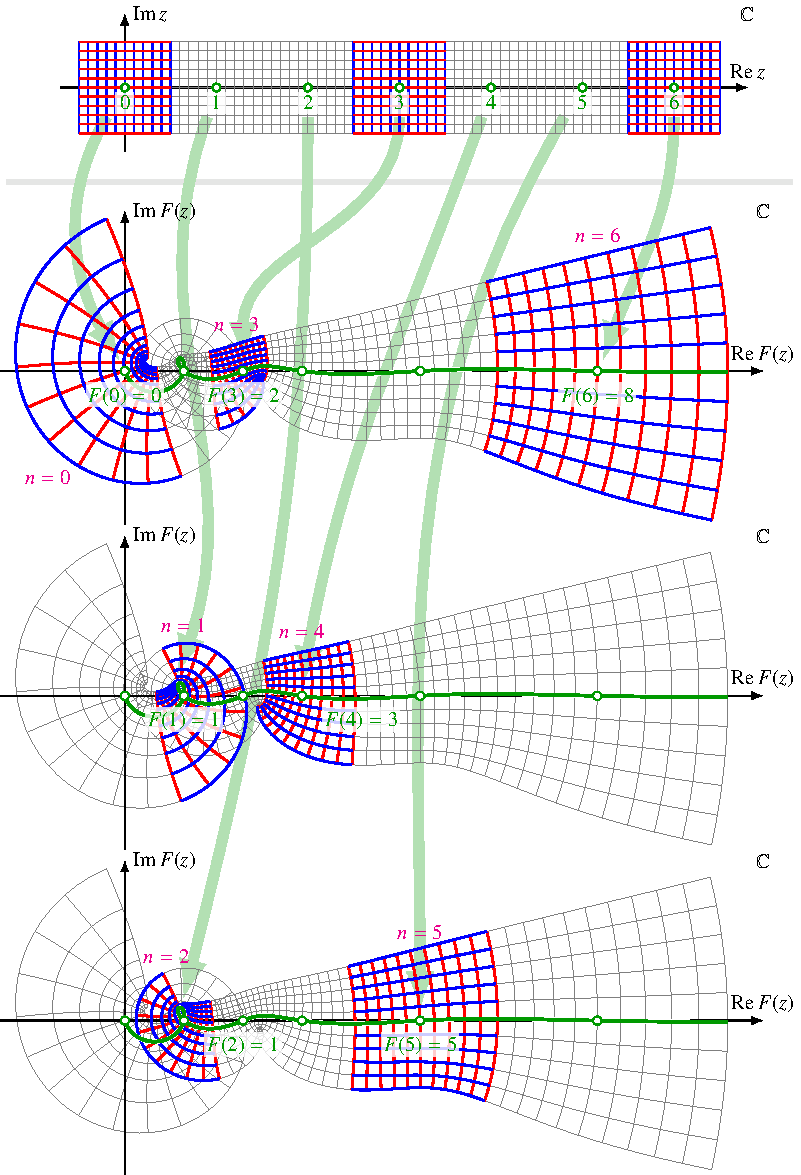
\includegraphics[width=0.82\textwidth]{chapters/040-rekursion/images/fibonacci.pdf}
\caption{Komplexe Fibonacci-Zahlen-Funktion $F(z)$ von
\eqref{buch:rekursion:linear:fibonaccifunktion}
dargestellt als Abbildung $\mathbb{C}\to\mathbb{C}$.
Die ganzzahligen $z$ werden auf die wohlbekannten Fibonacci-Zahlen
abgebildet.
Zur besseren Lesbarkeit wird der Wertebereich dreimal dargestellt,
damit die Bilder der einzelnen reellen Teilintervalle in verschiedene
Wertebereich-Bilder verteilt werden können.
$x$-Werte zwischen $3n-\frac12$ und $3n+\frac12$ werden im obersten
Bildbereich dargestellt, solche zwischen $3n+\frac12$ und $3n+\frac32$ 
im mittleren und schliesslich solche zwischen $3n+\frac32$ und $3n+\frac52$
im untersten.
Die reelle Achse wird auf die grüne Kurve abgebildet.
\label{buch:rekursion:linear:fibonaccigraph}}
\end{figure}
Abbildung~\eqref{buch:rekursion:linear:fibonaccigraph} zeigt die Abbildung
$z\mapsto F(z)$.
Allerdings sind die Funktionen
\[
F_{kl}(z)
=
\frac{1}{\sqrt{5}}
\varphi^ze^{2k\pi iz}
-
\frac{1}{\sqrt{5}(-\varphi)^z} e^{2l\pi z}
\]
ebenfalls Lösungen der Differenzengleichung mit den gleichen 
Anfangswerten.




%
% hypergeometrisch.tex
%
% (c) 2021 Prof Dr Andreas Müller, OST Ostschweizer Fachhochschule
%
\section{Hypergeometrische Funktionen
\label{buch:rekursion:section:hypergeometrische-funktion}}
\rhead{Hypergeometrische Funktionen}
Kann man eine Formel für die Lösung $S_n$ der lineare Differenzengleichung
\[
n^3S_{n}
=
16(n-{\textstyle\frac12})(2n^2-2n+1)S_{n-1}
-256(n-1)^3S_3
\]
mit Anfangswerten $S_0=1$ und $S_1=8$ angeben?
Dies scheint auf den ersten Blick unmöglich kompliziert, man kann aber
zeigen, dass
\[
S_n
=
\sum_{k=0}^n 
\binom{2n-2k}{n-k}^2 \binom{2k}{k}^2
\]
gilt (\cite[p.~xi]{buch:ab}).
Die Lösung ist also eine Summe von Summanden, die sehr viel einfacher
aussehen und vor allem die besondere Eigenschaft haben, dass die
Quotienten aufeinanderfolgender Terme rationale Funktionen von von $k$
sind.
% XXX Quotient berechnen

Eine besonders simple solche Funktion ist die geometrische Reihe, die
im Abschnitt~\ref{buch:rekursion:hypergeometrisch:geometrisch}
in Erinnerung gerufen wird.
Abschnitt~\ref{buch:rekursion:hypergeometrisch:reihen}
definiert den Begriff der hypergeometrischen Reihe und zeigt, 
wie sie in eine Standardform gebracht werden können.
In Abschnitt~\ref{buch:rekursion:hypergeometrisch:beispiele}
schliesslich wird an Hand von Beispielen gezeigt, wie bekannte
Funktionen als hypergeometrische Funktionen interpretiert werden können.

\subsection{Die geometrische Reihe
\label{buch:rekursion:hypergeometrisch:geometrisch}}
Die besonders einfache Potenzreihe
\[
f(q)
=
\sum_{k=0}^\infty aq^k
\]
heisst die {\em geometrische Reihe}.
Die Partialsummen 
\[
S_n
=
\sum_{k=0}^n aq^k
\]
kann mit der Differenz
\begin{equation}
(1-q)S_n
=
S_n - qS_n
=
\sum_{k=0}^n aq^k
-
\sum_{k=1}^{n+1} aq^k
=
a -aq^{n+1}
\label{buch:rekursion:hypergeometrisch:eqn:qsumme}
\end{equation}
berechnet werden, die man nach
\begin{equation}
S_n 
=
a\frac{1-q^{n+1}}{1-q}
\label{buch:rekursion:hypergeometrisch:eqn:geomsumme}
\end{equation}
auflösen kann.

Fü $q<1$ geht $q^n\to 0$ und damit konvergiert
$S_n$  gegen
\[
\sum_{k=0}^\infty aq^k
=
a\frac{1}{1-q}.
\]

Die geometrische Reihe ist charakterisiert dadurch, dass aufeinanderfolgende
Terme den gleichen Quotienten
\[
\frac{aq^{k+1}}{aq^k}
=
q
\]
haben.
Die Berechnung der Summe in 
\eqref{buch:rekursion:hypergeometrisch:eqn:qsumme}
beruht darauf, dass die Multiplikation mit $q$ einen ``anderen''
Teil der Summe ergibt, der sich in der Differenze weghebt.

\subsection{Hypergeometrische Reihen
\label{buch:rekursion:hypergeometrisch:reihen}}
Es ist plausibel, dass eine etwas lockerere Bedingung an die
Quotienten aufeinanderfolgender Terme einer Reihe immer noch
ermöglichen wird, interessante Aussagen über die durch die
Reihe beschriebenen Funktionen zu machen.

\begin{definition}
Eine Reihe
\[
f(x) = \sum_{k=0}^\infty a_k x^k
\]
heisst {\em hypergeometrisch}, wenn der Quotient aufeinanderfolgender
Koeffizienten eine rationale Funktion von $k$ ist,
wenn also
\[
\frac{a_{k+1}}{a_k}
=
\frac{p(k)}{q(k)}
\]
mit Polynomen $p(k)$ und $q(k)$ ist.
\end{definition}

Die geometrische Reihe ist natürlich eine hypergeometrische Reihe,
wobei $p(k)/q(k)=1$ ist.
Etwas interessanter ist die Exponentialfunktion, durch die Taylor-Reihe
\[
e^x = \sum_{k=0}^\infty \frac{x^k}{k!}
\]
dargestellt werden kann.
Der Quotient aufeinanderfolgender Koeffizienten ist
\[
\frac{a_{k+1}}{a_k}
=
\frac{1/(k+1)!}{1/k!}
=
\frac{k!}{(k+1)!}
=
\frac{1}{k+1},
\]
eine rationale Funktion mit Zählergrad $0$ und Nennergrad $1$.

Die Kosinus-Funktion wird durch die Taylor-Reihe
\[
\cos x = \sum_{k=0}^\infty \frac{(-1)^k}{(2k)!} x^{2k}
\]
dargestellt.
Als Potenzreihe in $x$ kann die Kosinus-Reihe nicht hypergeometrisch sein,
die ungeraden Koeffizienten verschwinden und damit undefinierte
Quotienten haben.
Als Reihe in $z=x^2$ ist aber
\[
\sum_{k=0}^\infty \frac{(-1)^k}{(2k)!} z^k
\qquad\Rightarrow\qquad
a_k = \frac{(-1)^k}{(2k)!}
\]
hypergeometrisch, weil der Quotient aufeinanderfolgender Koeffizienten
\[
\frac{a_{k+1}}{a_k}
=
\frac{(-1)^{k+1}}{(2k+2)!}\cdot \frac{(2k)!}{(-1)^k}
=
-\frac{1}{(2k+2)(2k+1)},
\]
eine rationale Funktion mit Zählergrad $0$ und Nennergrad $2$.
Es gibt also eine hypergeometrische Reihe $f(z)$ derart, dass
$\cos x = f(x^2)$ ist.

Seien $p(k)$ und $q(k)$ zwei Polynome derart, dass
\[
\frac{a_{k+1}}{a_k} = \frac{p(k)}{q(k)}.
\]
Daraus lässt sich der Koeffizient $a_{k+1}$ als
\begin{equation}
a_{k+1}
=
\frac{p(k)}{q(k)}
\cdot
a_k
=
\frac{p(k)}{q(k)}
\cdot
\frac{p(k-1)}{q(k-1)}
\cdot
a_{k-1}
=\dots=
\frac{p(k)}{q(k)}
\frac{p(k-1)}{q(k-1)}
\cdots
\frac{p(1)}{q(1)}
\frac{p(0)}{q(0)}
a_0
\label{buch:rekursion:hypergeometrisch:ak+1}
\end{equation}
berechnen.
Alle Koeffizienten haben also den Faktor $a_0=f(0)$ gemeinsam.

Die Produkte von Quotienten $p(k)/q(k)$ sollen jetzt weiter
vereinfacht werden.
Sei $n$ der Grad von $p(k)$ und $m$ der Grad von $q(k)$.
Dazu nehmen wir an, dass $a_i$, $i=1,\dots,n$ die Nullstellen von $p(k)$ sind
und $b_j$, $j=1,\dots,m$ die Nullstellen von $q(k)$, dass man also
die Polynome als
\begin{align*}
p(k) &= x(k-a_1)(k-a_2)\cdots(k-a_n)
\\
q(k) &= (k-b_1)(k-b_2)\cdots(k-b_m)
\end{align*}
schreiben kann.
Der Faktor $x$ ist nötig, weil die Polynome $p(k)$ und $q(k)$ nicht
notwendigerweise normiert sind.

Um das Produkt der Quotienten zu vereinfachen, nehmen wir für den Moment
an, dass Zähler und Nenner vom Grad $n=m=1$ ist.
Dann ist nach 
\eqref{buch:rekursion:hypergeometrisch:ak+1}
\[
a_{k}
=
x^{k}
\frac{
(k-1-a_1) \cdots (2-a_1)(1-a_1)(0-a_1)
}{
(k-1-b_1) \cdots (2-b_1)(1-b_1)(0-b_1)
}
=
\frac{(-a_1)_k}{(-b_1)_k} x^k.
\]
Die Koeffizienten können daher als Quotienten von Pochhammer-Symbolen
geschrieben werden.
Für Polynome $p(k)$ und $q(k)$ höheren Grades sind die Koeffizienten
von der Form
\[
a_k
=
\frac{(-a_1)_k(-a_2)_k\cdots (-a_n)_k}{(-b_1)_k(-b_2)_k\cdots(-b_m)_k}
x^ka_0.
\]
Jede hypergeometrische Reihe kann daher in der Form
\[
a_0
\sum_{k=0}^\infty
\frac{(-a_1)_k(-a_2)_k\cdots (-a_n)_k}{(-b_1)_k(-b_2)_k\cdots(-b_m)_k}
x^k
\]
geschrieben werden.

\begin{definition}
\label{buch:rekursion:hypergeometrisch:def}
Die hypergeometrische Funktion
$\mathstrut_pF_q$ ist definiert durch die Reihe
\[
\mathstrut_pF_q
\biggl(
\begin{matrix}
a_1,\dots,a_p\\
b_1,\dots,b_q
\end{matrix}
;
x
\biggr)
=
\mathstrut_pF_q(a_1,\dots,a_p;b_1,\dots,b_q;x)
=
\sum_{k=0}^\infty
\frac{(a_1)_k\cdots(a_p)_k}{(b_1)_k\cdots(b_q)_k}\frac{x^k}{k!}.
\]
\end{definition}

Da $(1)_k=k!$ hätte die Definition den Nenner $k!$ in der Reihe
auch durch eines der Pochhammer-Symbole ausdrücken können.
Wird dieser Nenner nicht gebraucht, kann man ihn durch einen 
zusätzlichen Faktor $(1)_k$ im Zähler des Bruchs von Pochhammer-Symbolen
kompensieren, wodurch sich der Grad $p$ des Zählers natürlich um $1$
erhöht.

Die oben analysierte Summe $S$ kann mit der Definition als
\[
S
=
a_0
\,
\mathstrut_{n+1}F_m \biggl(
\begin{matrix}
-a_1,-a_2,\dots,-a_n,1\\
-b_1,-b_2,\dots,-a_m
\end{matrix}; x
\biggr)
\]
beschrieben werden.

\subsection{Beispiele von hypergeometrischen Funktionen
\label{buch:rekursion:hypergeometrisch:beispiele}}
Viele der bekannten Reihenentwicklungen häufig verwendeter Funktionen
lassen sich durch die hypergeometrischen Funktionen von
Definition~\ref{buch:rekursion:hypergeometrisch:def} ausdrücken.
In diesem Abschnitt werden einige Beispiel dazu gegeben.

\subsubsection{Die geometrische Reihe}
In der geometrischen Reihe fehlt der Nenner $k!$, es braucht
daher einen Term $(1)_k$ im Zähler, um den Nenner zu kompensieren.
Somit ist die geometrische Reihe
\[
\frac{a}{1-x}
=
\sum_{k=0}^\infty
ax^k
=
a\sum_{k=0}^\infty
\frac{(1)_k}{1}
\frac{x^k}{k!}
=
a\,\mathstrut_1F_0(1,x).
\]

\subsubsection{Exponentialfunktion}
Die Exponentialfunktion ist die Reihe
\[
e^x = \sum_{k=0}^\infty \frac{x^k}{k!}.
\]
In diesem Fall werden keine Quotienten von Pochhammer-Symbolen
benötigt, es ist daher
\[
e^x = \mathstrut_0F_0(x).
\]

\subsubsection{Wurzelfunktion}
Die Wurzelfunktion $x\mapsto \sqrt{x}$ hat keine Taylor-Entwicklung
in $x=0$, aber die Funktion $x\mapsto\sqrt{1+x}$ hat die Taylor-Reihe
\[
\sqrt{1+x}
=
1
+
\frac12 x
-
\frac{1\cdot 1}{2\cdot 4}x^2
+
\frac{1\cdot 1\cdot 3}{2\cdot 4\cdot 6}x^3
-
\frac{1\cdot 1\cdot 3\cdot 5}{2\cdot 4\cdot 6\cdot 8}x^4
+
\dots
\]
Um die Verbindung zu einer hypergeometrischen Funktion herzustellen,
müssen wir den Term $x^k/k!$ abspalten.
Dann wird
\begin{align*}
\sqrt{1+x}
&=
1
+
\frac12 \frac{x}{1!}
-
\frac{1\cdot 1}{2^2}\frac{x^2}{2!}
+
\frac{1\cdot 1\cdot 3}{2^3}\frac{x^3}{3!}
-
\frac{1\cdot 1\cdot 3\cdot 5}{2^4}\frac{x^4}{4!}
+
\dots
\\
&=
1
+
\frac12 \cdot\frac{x}{1!}
-
\frac{1}{2}\cdot \frac{1}{2}\cdot\frac{x^2}{2!}
+
\frac{1}{2}\cdot \frac{1}2\cdot \frac{3}{2}\cdot\frac{x^3}{3!}
-
\frac{1}{2}\cdot \frac{1}{2}\cdot \frac{3}{2}\cdot \frac{5}{2}\cdot\frac{x^4}{4!}
+
\dots
\end{align*}
Es ist noch etwas undurchsichtig, warum die ersten beiden Terme
das gleiche Vorzeichen haben und warum der Faktor $\frac12$ in jedem
Term zweimal vorkommt.
Diese Unklarheit kann jedoch beseitigt werden, wenn man den ersten
Faktor als $-\frac12$ schreibt:
\begin{align*}
\sqrt{1+x}
&=
1
-
\biggl(-\frac12\biggr)\cdot\frac{x}{1!}
+
\biggl(-\frac{1}{2}\biggr)\cdot \frac{1}{2}\cdot\frac{x^2}{2!}
-
\biggl(-\frac{1}{2}\biggr)\cdot \frac{1}2\cdot \frac{3}{2}\cdot\frac{x^3}{3!}
+
\biggl(-\frac{1}{2}\biggr)\cdot \frac{1}{2}\cdot \frac{3}{2}\cdot \frac{5}{2}\cdot\frac{x^4}{4!}
+
\dots
\\
&=
1 + 
\biggl(-\frac12\biggr)\cdot\frac{-x}{1!}
+
\biggl(-\frac{1}{2}\biggr)\cdot \frac{1}{2}\cdot\frac{(-x)^2}{2!}
+
\biggl(-\frac{1}{2}\biggr)\cdot \frac{1}2\cdot \frac{3}{2}\cdot\frac{(-x)^3}{3!}
+
\biggl(-\frac{1}{2}\biggr)\cdot \frac{1}{2}\cdot \frac{3}{2}\cdot \frac{5}{2}\cdot\frac{(-x)^4}{4!}
+
\dots
\end{align*}
Die Koeffizienten sind aufsteigende Produkte mit $k$ Faktoren, die alle bei
$-\frac12$ beginnen, sie können daher als Pochhammer-Symbole $(-\frac12)_k$
geschrieben werden.
Die Wurzelfunktion ist daher die hypergeometrische Funktion
\[
\sqrt{1\pm x}
=
\sum_{k=0}^\infty
\biggl(-\frac12\biggr)_k \frac{(-x)^k}{k!}
=
\mathstrut_1F_0(-{\textstyle\frac12};\mp x).
\]

\subsubsection{Logarithmusfunktion}
Für $x\in (-1,1)$ konvergiert die Taylor-Reihe
\[
\log(1+x)
=
x-\frac{x^2}{2}+\frac{x^3}{3}-\frac{x^4}{4}+\dots
\]
der Logarithmusfunktion im Punkt $x=0$.
Die Reihe beginnt nicht mit einem konstanten Term, daher klammern wir
zunächst einen Faktor $x$ aus:
\[
\log(1+x)
=
x\cdot
\biggl(
1-\frac{x}{2}+\frac{x^2}{3}-\frac{x^3}{4}+\dots
\biggr)
\]
Um dies in die Form einer hypergeometrischen Funktion zu bringen,
muss zunächst wieder der Nenner $k!$ hergestellt werden.
\begin{align*}
\log(1+x)
&=
x\cdot\biggl(
1
- \frac{1!}{2} \frac{x}{1!}
+ \frac{2!}{3} \frac{x^2}{2!} 
- \frac{3!}{4} \frac{x^3}{3!}+\dots
\biggr).
\intertext{Den Nenner $k+1$ kann man als Quotienten $k!/(k+1)!$ erhalten,
also}
\log(1+x)
&=
x\cdot\biggl(
1
- \frac{(1!)^2}{2!} \frac{x}{1!}
+ \frac{(2!)^2}{3!} \frac{x^2}{2!} 
- \frac{(3!)^2}{4!} \frac{x^3}{3!}+\dots
\biggr).
\end{align*}
Die Fakultät
\[
(k+1)!
=
1\cdot 2 \cdot 3 \cdot\ldots\cdot k\cdot (k+1)
=
2 \cdot (2 + 1) \cdot (2+2) \cdot\ldots\cdot (2+k-2) \cdot (2+k-1)
=
(2)_{k}
\]
ist auch ein Pochhammer-Symbol, so dass die Logarithmusfunktion
zur hypergeometrischen Funktion
\[
\log(1+x)
=
x\cdot\biggl(
1
+ \frac{(1)_1(1)_1}{(2)_1} \frac{(-x)}{1!}
+ \frac{(1)_2(1)_2}{(2)_2} \frac{(-x)^2}{2!} 
+ \frac{(1)_3(1)_3}{(2)_2} \frac{(-x)^3}{3!}+\dots
\biggr)
=
x\cdot
\mathstrut_2F_1\biggl(\begin{matrix}1,1\\2\end{matrix};-x\biggr).
\]


\subsubsection{Trigonometrische Funktionen}
Die Kosinus-Funktion wurde bereits als hypergeometrische Funktion erkannt,
im Folgenden soll dies auch noch für die Sinus-Funktion
durchgeführt werden.
Die Taylor-Reihe der Sinus-Funktion im Punkt $0$ ist
\begin{align*}
\sin x
&=
x-\frac{x^3}{3!}+\frac{x^5}{5!}-\frac{x^7}{7!}+\dots
\end{align*}
In dieser Reihe fehlen die geraden Potenzen, wir Klammern daher einen
Faktor $x$ aus und schreiben den Rest als eine Funktion von $-x^2$
\begin{align*}
\sin x
&=
x
\biggl(
1+\frac{-x^2}{3!}+\frac{(-x^2)^2}{5!}-\frac{(-x^2)^3}{7!}+\dots
\biggr)
=
x f(-x^2).
\end{align*}
Die Funktion $f(z)$ soll jetzt als hypergeometrische Funktion geschrieben
werden.
Dazu muss zunächst wieder der Nenner $k!$ wiederhergestellt werden:
\[
f(z)
=
1
+
\frac{1!}{3!}\cdot \frac{z}{1!}
+
\frac{2!}{5!}\cdot \frac{z^2}{2!}
+
\frac{3!}{7!}\cdot \frac{z^3}{3!}
+
\dots
\]
Die Koeffizienten $k!/(2k+1)!$ müssen jetzt durch Pochhammer-Symbole
mit jeweils $k$ Faktoren ausgedrückt werden.
Dazu muss die Fakultät $(2k+1)!$ in zwei Produkte
\[
(2k+1)
=
2\cdot 3 \cdot 4\cdot 5\cdot \ldots \cdot 2k \cdot (2k+1)
=
(2\cdot 4 \cdot 6\cdot\ldots\cdot 2k)
\cdot
(3\cdot 5\cdot 7\cdot \ldots \cdot (2k+1))
\]
aufgespaltet werden.
Diese Produkte haben zwar $k$-Faktoren, aber sie sind keine
Pochhammer-Symbole, weil die Differenz aufeinanderfolgender Faktoren 
jeweils $2$ ist.
Wir dividieren die geraden Faktoren durch $2$ und dividieren die 
ungeraden durch $2$, dadurch ändert sich das Produkt nicht und wird
\[
(2k+1)!
=
(1\cdot2\cdot3\cdot\ldots\cdot k)
\cdot
\biggl(
\frac{3}{2}\cdot
\frac{5}{2}\cdot
\frac{7}{2}\cdot
\ldots\cdot
\frac{2k+1}{2}
\biggr)
=
(1)_k\cdot \biggl(\frac{3}{2}\biggr)_k
\]
Setzt man dies in die Reihe ein, wird
\[
f(z)
=
\sum_{k=0}^\infty
\frac{(1)_k}{(1)_k\cdot (\frac{3}{2})_k}
z^k
=
\mathstrut_1F_2(1;1,\frac{3}{2};z).
\]
Damit lässt sich die Sinus-Funktion als
\begin{equation}
\sin x
=
x\,\mathstrut_1F_2\biggl(\begin{matrix}1\\1,\frac32\end{matrix};-x^2\biggr)
=
x\,\mathstrut_1F_2\biggl(\begin{matrix}\text{---}\\\frac32\end{matrix};-x^2\biggr)
\label{buch:rekursion:hypergeometrisch:eqn:sinhyper}
\end{equation}
durch eine hypergeometrische Funktion ausdrücken.

\subsubsection{Hyperbolische Funktionen}
Die für die Sinus-Funktion angewendete Methode lässt sich auch
auf die Funktion 
\begin{align*}
\sinh x
&=
\sum_{k=0}^\infty \frac{x^{2k+1}}{(2k+1)!}
\\
&=
x
\,
\biggl(
1+\frac{x^2}{3!} + \frac{x^4}{5!}+\frac{x^6}{7!}+\dots
\biggr)
\\
&=
xf(-x^2)
=
x\,\mathstrut_1F_2\biggl(
\begin{matrix}1\\1,\frac{3}{2}\end{matrix}
;x^2
\biggr)
=
x\,\mathstrut_0F_1\biggl(
\begin{matrix}\text{---}\\,\frac{3}{2}\end{matrix}
;x^2
\biggr).
\end{align*}
Bis auf das Vorzeichen des Arguments der hypergeometrischen Funktion
ist diese Darstellung identisch mit der von $\sin x$.
Dies illustriert die Rolle der hypergeometrischen Funktionen als
``grosse Vereinheitlichung'' der bekannten speziellen Funktionen.

%
% Ableitung und Stammfunktion
%
\subsection{Ableitung und Stammfunktion hypergeometrischer Funktionen}
Sowohl Ableitung wie auch Stammfunktion einer hypergeometrischen
Funktion lässt sich immer durch hypergeometrische Reihen ausdrücken.

\subsubsection{Ableitung}
Wir gehen aus von der Funktion
\begin{equation}
f(x)
=
\mathstrut_nF_m\biggl(
\begin{matrix}a_1,\dots,a_n\\b_1,\dots,b_m\end{matrix};
x\biggr)
=
\sum_{k=0}^\infty
\frac{
(a_1)_k\cdot\ldots\cdot(a_n)_k
}{
(b_1)_k\cdot\ldots\cdot(b_m)_k
}
\frac{x^k}{k!}.
\label{buch:rekursion:hypergeometrisch:eqn:f}
\end{equation}
Die Ableitung von $f(x)$ ist
\[
f'(x)
=
\sum_{k=0}^\infty
\frac{
(a_1)_k\cdot\ldots\cdot(a_n)_k
}{
(b_1)_k\cdot\ldots\cdot(b_m)_k
}
\frac{x^{k-1}}{(k-1)!}
=
\sum_{k=1}^\infty
\frac{
(a_1)_{k+1}\cdot\ldots\cdot(a_n)_{k+1}
}{
(b_1)_{k+1}\cdot\ldots\cdot(b_m)_{k+1}
}
\frac{x^k}{k!}.
\]
Der Koeffizient besteht zwar aus lauter Pochhammer-Symbolen, aber sie
haben jeweils zu einen Faktor zuviel.
Indem man den jeweils ersten Faktor ausklammert, kann man die
Terme wieder in die Form einer hypergeometrischen Reihe bringen.
\begin{align*}
f'(x)
&=
\sum_{k=1}^\infty
\frac{
a_1(a_1)_{k}\cdot\ldots\cdot a_n(a_n)_{k}
}{
b_1(b_1)_{k}\cdot\ldots\cdot b_m(b_m)_{k}
}
\frac{x^k}{k!}
\\
&=
\sum_{k=1}^\infty
\frac{
a_1\cdot\ldots\cdot a_n
}{
b_1\cdot\ldots\cdot b_m
}
\frac{
(a_1+1)_{k}\cdot\ldots\cdot(a_n+1)_{k}
}{
(b_1+1)_{k}\cdot\ldots\cdot(b_m+1)_{k}
}
\frac{x^k}{k!}
\\
&=
\frac{
a_1\cdot\ldots\cdot a_n
}{
b_1\cdot\ldots\cdot b_m
}
\,
\mathstrut_nF_m\biggl(
\begin{matrix}a_1+1,\dots,a_n+1\\b_1+1,\dots,b_m+1\end{matrix};
x\biggr).
\end{align*}

\begin{beispiel}
Die Kosinus-Funktion
\[
\cos x
=
1 - \frac{x^2}{2!} + \frac{x^4}{4!} - \frac{x^6}{6!} + \dots
=
\sum_{k=0}^\infty
\frac{(-1)^k}{(2k)!}x^{2k}
\]
kann wie folgt als hypergeometrische Funktion geschrieben werden.
Der Nenner hat $2k$ Faktoren, er muss also aus zwei Pochhammer-Symbolen
zusammengesetzt werden.
Dazu muss er erst um den Faktor $2^{2k}$ gekürzt werden, was
\[
\frac{(2k)!}{2^{2k}}
=
\frac12\cdot\frac32\cdot\frac52\cdot\ldots\cdot\frac{2k-1}2
\cdot
\frac22\cdot\frac42\cdot\frac62\cdot\ldots\cdot\frac{2k}2
=
({\textstyle\frac12})_k\cdot k!.
\]
Damit kann jetzt die Kosinus-Funktion als
\begin{align*}
\cos x
&=
\sum_{k=0}^\infty
\frac{2^k}{(2k)!}\biggl(\frac{-x^2}{4}\biggr)^k
=
\sum_{k=0}^\infty
\frac{1}{(\frac12)_k}
\frac{1}{k!}\biggl(\frac{-x^2}{4}\biggr)^k
=
\mathstrut_0F_1\biggl(;\frac12;-\frac{x^2}4\biggr)
\end{align*}
geschrieben werden kann.

Die Ableitung der Kosinus-Funktion ist daher
\begin{align*}
\frac{d}{dx} \cos x
&=
\frac{d}{dx}
\mathstrut_0F_1\biggl(;\frac12;-\frac{x^2}4\biggr)
=
\frac{1}{\frac12}
\,
\mathstrut_0F_1\biggl(;\frac32;-\frac{x^2}4\biggr)
\cdot\biggl(-\frac{x}2\biggr)
=
-x
\,
\mathstrut_0F_1\biggl(;\frac32;-\frac{x^2}4\biggr)
\intertext{Dies stimmt mit der in
\eqref{buch:rekursion:hypergeometrisch:eqn:sinhyper}
gefundenen Darstellung der Sinusfunktion mit Hilfe der hypergeometrischen
Funktion $\mathstrut_0F_1$ überein, es ist also wie erwartet}
&=-\sin x.
\qedhere
\end{align*}
\end{beispiel}

\subsubsection{Stammfunktion}
Eine Stammfunktion kann man auf die gleiche Art und Weise wie
die Ableitung finden.
Termweises Integrieren der Funktion
\eqref{buch:rekursion:hypergeometrisch:eqn:f}
ergibt
\begin{align}
\int f(x)\,dx
&=
\sum_{k=0}^\infty
\frac{
(a_1)_k\cdot\ldots\cdot(a_n)_k
}{
(b_1)_k\cdot\ldots\cdot(b_m)_k
}
\frac{x^{k+1}}{(k+1)!}.
\notag
\intertext{Wieder muss man die Pochhammer-Symbole durch solche mit
einem zusätzlichen Faktor schreiben.
Dies ist möglich, wenn keiner der Parameter $a_i=1$ und $b_j=1$
ist.
Die Stammfunktion wird daher
}
&=
\sum_{k=1}^\infty
\frac{
(a_1-1)(a_1)_k
\cdot\ldots\cdot
(a_n-1)(a_n)_k
}{
(b_1-1)(b_1)_k
\cdot\ldots\cdot
(b_m-1)(b_m)_k
}
\frac{x^k}{k!}
\notag
\\
&=
\sum_{k=1}^\infty
\frac{
(a_1-1)_{k+1}
\cdot\ldots\cdot
(a_n-1)_{k+1}
}{
(b_1-1)_{k+1}
\cdot\ldots\cdot
(b_m-1)_{k+1}
}
\frac{x^k}{k!}
\label{buch:rekursion:hypergeometrisch:eqn:stammfunktion:summe}
\\
&=
\mathstrut_nF_m\biggl(
\begin{matrix}
a_1-1,\dots,a_n-1\\
b_1-1,\dots,b_m-1
\end{matrix}
;x
\biggr)
-
\frac{(a_1-1)\dots(a_n-1)}{(b_1-1)\dots(b_m-1)}.
\notag
\end{align}
Der Term auf der rechten Seite kompensiert den konstanten
Term, der in der hypergeometrischen Funktion $\mathstrut_nF_m$
vorkommt, aber nicht in der
Summe~\eqref{buch:rekursion:hypergeometrisch:eqn:stammfunktion:summe}.




\section*{Übungsaufgaben}
\rhead{Übungsaufgaben}
\aufgabetoplevel{chapters/040-rekursion/uebungsaufgaben}
\begin{uebungsaufgaben}
%\uebungsaufgabe{0}
\uebungsaufgabe{401}
\uebungsaufgabe{402}
\uebungsaufgabe{403}
\end{uebungsaufgaben}

